\section{Metrics of 6 networks}
In this section I will present some statistics about the 6 chosen networks. The results will be presented in tables. It is also noteworthy to reiterate that Gephi does not display nodes if their degree is 0.

\begin{table}
    \centering
    \begin{tabular}{|c|c|c|c|c|c|c|c|}
        \hline
        \textbf{Metric} & \textbf{Net. 1} & \textbf{Net. 2} & \textbf{Net. 3} & \textbf{Net. 4} & \textbf{Net. 5} & \textbf{Net. 7} \\
        \hline
        Num. Nodes & 59 & 55 & 52 & 41 & 29 & 59 \\
        \hline
        Num. Edges & 427 & 124 & 80 & 54 & 34 & 216 \\
        \hline
        Density & 0.125 & 0.084 & 0.060 & 0.066 & 0.084 & 0.126 \\
        \hline
        Avg. Clust. Coef. & 0.375 & 0.412 & 0.482 & 0.583 & 0.620 & 0.542 \\
        \hline
        Num. Nodes SCC & 49 & - & - & - & - & - \\
        \hline
        Num. Nodes WCC & 58 & - & - & - & - & - \\
        \hline
        Num. Nodes CC & - & 52 & 42 & 20 & 10 & 59 \\
        \hline
        Avg. Path Len. SCC & 2.599 & - & - & - & - & - \\
        \hline
        Avg. Path Len. CC & - & 3.143 & 4.234 & 2.857 & 1.711 & 2.654 \\
        \hline
        Diameter of SCC & 7 & - & - & - & - & - \\
        \hline
        Diameter of CC & - & 7 & 11 & 6 & 4 & 6 \\
        \hline
    \end{tabular}
    \caption{Network statistics}
    \label{table:1}
\end{table}

\subsection{Number of nodes}
The number of nodes of each graph will be the amount of people who have at least one edge connecting them to another person.

\subsection{Number of edges}
The number of edges of each graph will be the amount of connections that exist between each person for each question.

\subsection{Edge density}
Graph density tells us how connected nodes are between each other. For undirected graphs, this metric can be calculated as
\begin{equation}
    D_{undirected} = \frac{2|E|}{|N|(|N|-1)}
    \label{equation:dir_density}
\end{equation}
and the density for directed graphs is defined as
\begin{equation}
    D_{directed} = \frac{|E|}{|N|(|N    |-1)}
    \label{equation:undir_density}
\end{equation}
where $E$ is the number of edges and $V$ is the number of nodes in the graph.

\subsection{Degree distribution}
The degree distribution of a graph allows us to grasp how deeply connected the nodes are. Figure \ref{fig:4} pictures the degree distributions for the 6 chosen networks.
\begin{figure}
    \centering
    \subfloat[\centering Network 1]{{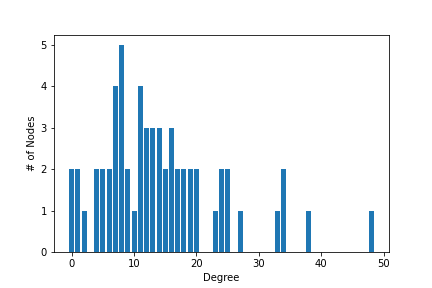
\includegraphics[width=0.45\textwidth]{img/net_0_degree_distribution.png}}}
    \qquad
    \subfloat[\centering Network 2]{{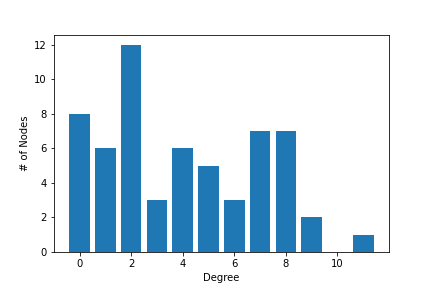
\includegraphics[width=0.45\textwidth]{img/net_1_degree_distribution.png}}}
    \qquad
    \subfloat[\centering Network 3]{{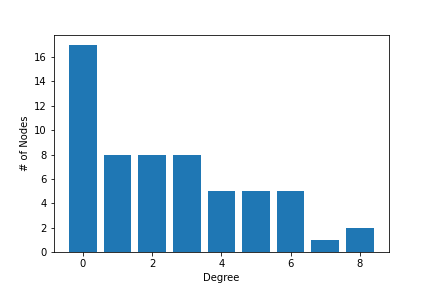
\includegraphics[width=0.45\textwidth]{img/net_2_degree_distribution.png}}}
    \qquad
    \subfloat[\centering Network 4]{{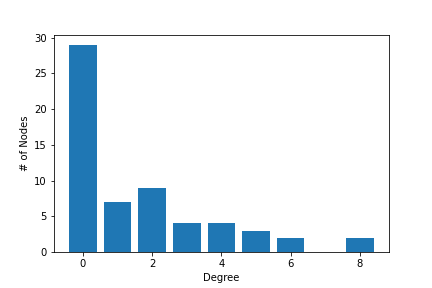
\includegraphics[width=0.45\textwidth]{img/net_3_degree_distribution.png}}}
    \qquad
    \subfloat[\centering Network 5]{{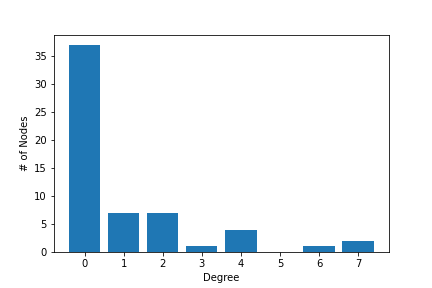
\includegraphics[width=0.45\textwidth]{img/net_4_degree_distribution.png}}}
    \qquad
    \subfloat[\centering Network 7]{{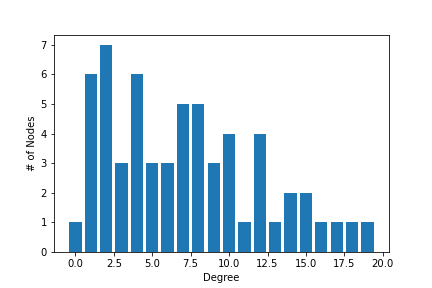
\includegraphics[width=0.45\textwidth]{img/net_6_degree_distribution.png}}}
    \caption{Degree distributions}
    \label{fig:4}
\end{figure}

\subsection{Average clustering coefficient}
The average clustering coefficient for a graph helps determine how transitive a relationship is. The clustering coefficient is defined as
\begin{equation}
    C_i = \frac{2e_i}{k_i(k_i-1)}
    \label{equation:clustering_coef}
\end{equation}
where $e_i$ is the number of edges between the neighbors of node $i$.

The average clustering coefficient of the graph is calculated as
\begin{equation}
    \left\langle C \right\rangle = \frac{1}{N}\sum_{i}^{N}C_i
    \label{equation:avg_clustering_coef}
\end{equation}
where $N$ is the number of nodes in the graph, and $C_i$ is the clustering coefficient of node $i$.

\subsection{Number of nodes in strongly connected component (SCC)}
The strongly connected component (SCC) metric can only be obtained from directed graphs. Since only the first network, then it is the only one that can provide this value. For networks 2 through 5, and 7, the values are from the connected components. Refer to table \ref{table:1} for the values.

\subsection{Number of nodes in weakly connected component (WCC)}
The weakly connected component (WCC) metric can only be obtained from directed graphs. Since only the first network, then it is the only one that can provide this value. For networks 2 through 5, and 7, the values are from the connected components. Refer to table \ref{table:1} for the values.

\subsection{Average path length in SCC}
The average path length metric indicates how far apart two nodes are from each other in the connected graph. In other words, how many jumps, in average, it takes to reach other nodes. For a directed graph, it is calculated as
\begin{equation}
    \left\langle d \right\rangle \equiv \frac{1}{2L_{max}}\sum_{i,j \neq i}d_{ij}
    \label{equation:dir_avg_path_len}
\end{equation}

For undirected graphs, it is calculated as
\begin{equation}
    \left\langle d \right\rangle \equiv \frac{1}{L_{max}}\sum_{i,j >  i}d_{ij}
    \label{equation:undir_avg_path_len}
\end{equation}

For networks 2 through 5, and 7, I calculated the average path length in the connected component because these networks are undirected graphs, thus not being possible to determine strongly connected components.

\subsection{Diameter of SCC}
This metric represents the maximum shortest distance between two nodes in a connected graph. It can be represented as
\begin{equation}
    diameter \equiv \max_{ij}d_{ij}
    \label{equation:diameter}
\end{equation}

For the first network, I collected the diameter of the strongly connected component. However, since all other networks are undirected graphs, I collected the diameter of the largest connected component.

\subsection{Community detection}
To detect communities in each of the chosen networks, I ran the Girvan--Newman algorithm, implemented in NetworkX. Figure \ref{fig:5} illustrates the communities in each network. The communities the algorithm found make sense, given that it ran by removing the edges with highest betweenness, separating the communities the edge held together. Also, by comparing with figures \ref{fig:1}, \ref{fig:2}, and \ref{fig:3}, we can see that the nodes with most connections between each other form a community the algorithm was able to find.
\begin{figure}[h!]
    \centering
    \subfloat[\centering Network 1]{{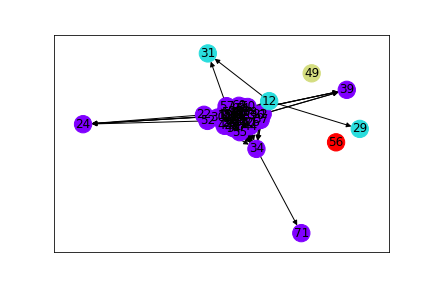
\includegraphics[width=0.45\textwidth]{img/net_0_communities.png}}}
    \qquad
    \subfloat[\centering Network 2]{{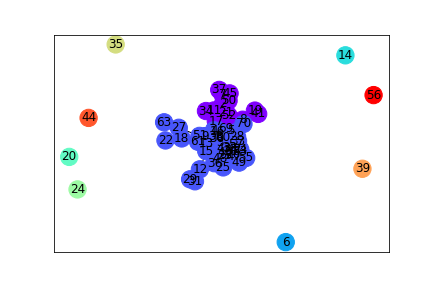
\includegraphics[width=0.45\textwidth]{img/net_1_communities.png}}}
    \qquad
    \subfloat[\centering Network 3]{{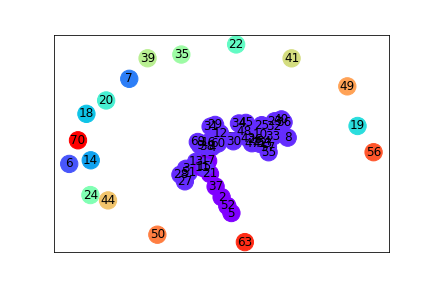
\includegraphics[width=0.45\textwidth]{img/net_2_communities.png}}}
    \qquad
    \subfloat[\centering Network 4]{{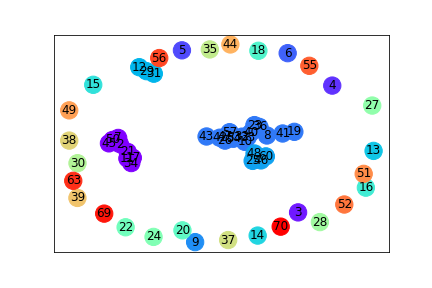
\includegraphics[width=0.45\textwidth]{img/net_3_communities.png}}}
    \qquad
    \subfloat[\centering Network 5]{{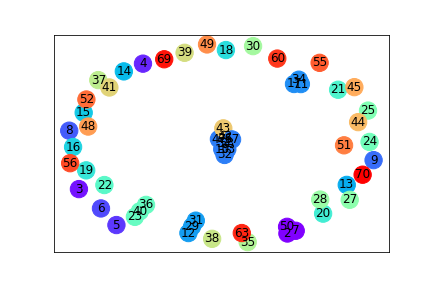
\includegraphics[width=0.45\textwidth]{img/net_4_communities.png}}}
    \qquad
    \subfloat[\centering Network 7]{{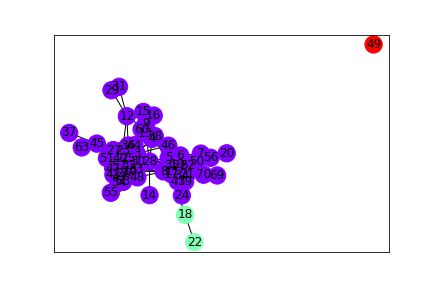
\includegraphics[width=0.45\textwidth]{img/net_6_communities.png}}}
    \caption{Detected Communities}
    \label{fig:5}
\end{figure}

\subsection{Centrality Measures}
Centrality tries to determine which node is the most central. The four centrality measures will be used to determine which node is the most important in each network. The measures are in-degree, out-degree, betweenness, and closeness. They will be explained as they are used.